% !TeX encoding = UTF-8
% !TeX spellcheck = en_GB

\newcommand{\doublequotes}[1]{``#1''}

\newcommand{\entity}[1]{{\color{red}#1}}
\newcommand{\attribute}[1]{{\color{Green}#1}}
\newcommand{\relationship}[1]{{\color{blue}#1}}

\newcommand{\page}[1]{{\color{red}#1}}
\newcommand{\component}[1]{{\color{Green}#1}}
\newcommand{\event}[1]{{\color{blue}#1}}
\newcommand{\action}[1]{{\color{brown}#1}}

\newcommand{\grey}[1]{{\color{gray}#1}}

\newcommand{\graycell}{\cellcolor[gray]{0.9}}

\NewDocumentCommand\ulverb{v}{\uline{\ttfamily#1}}

\documentclass[a4paper, dvipsnames]{article}

\pdfminorversion=7
\pdfcompresslevel=9
\pdfobjcompresslevel=2

\usepackage[hidelinks]{hyperref}
\usepackage[margin=60pt]{geometry}
\usepackage[T1]{fontenc}
\usepackage[utf8]{inputenc}
\usepackage[english]{babel}
\usepackage{array}
\usepackage{changepage}
\usepackage{graphicx}
\usepackage{minted}
\usepackage{multicol}
\usepackage[normalem]{ulem}
\usepackage[underline=false]{pgf-umlsd}
\usepackage{xcolor}
\usepackage{xparse}

\graphicspath{ {./images/} }

\setlength{\parindent}{0pt}
\newcolumntype{C}{>{\centering\arraybackslash} m{0.16\columnwidth} }

\title{\textbf{DocManager documentation}}
\author{Davide Figini and Riccardo Motta}
\date{A.Y. 2021 - 2022}

\hypersetup{
	pdftitle={DocManager documentation},
	pdfauthor={Davide Figini and Riccardo Motta}
}

\begin{document}

	\maketitle
	
	\section{Project's description}
	
	\begin{multicols}{2}
		A web application allows the online management of folders, subfolders and documents. The application supports user registration and login via a public page with appropriate forms. Registration check the uniqueness of the username. A folder has an owner, a name and a creation date and can (only) contains subfolders. A subfolder can (only) contain documents. A document has an owner, name, creation date, a summary and a type. When the uses accesses the application, a HOME PAGE appears containing a tree of its folders and subfolders. In the HOME PAGE the user can select a subfolder and access to a DOCUMENTS page which shows the list of documents of a subfolder. Each document in the list has two links: \textit{access} and \textit{move}. When the user selects the \textit{access} link, a DOCUMENT page appears showing all the data of the selected document. When the user selects the \textit{move} link, the HOME PAGE appears with the tree of folders and subfolders; in this case the page shows the message \doublequotes{You're moving the document X from the subfolder Y. Choose the destination subfolder}, the subfolder to which the document to move belongs is NOT selectable and it's name is highlighted (for example with a different colour). When the user selects the destination subfolder, the document is moved from the origin subfolder, to the destination one and the DOCUMENTS page appears showing the updated content of the destination subfolder. Every page, except from the HOME PAGE, contains a link to go back to the previous page. The application allows the user to logout. A DOCUMENT MANAGEMENT page reachable from the HOME PAGE allows the user to create a folder, a subfolder of an existing folder and a document inside a subfolder.
	\end{multicols}
	
	\subsection{Changes in the JavaScript version}
	
	\begin{multicols}{2}
		\begin{itemize}
			\item The registration check the syntactic validity of the email address and the equality between the fields \doublequotes{password} and \doublequotes{repeat password}, also client-side.
			\item After the login, the entire application is made of a single page.
			\item Every user interaction is manages without refreshing the whole page, but produces the asynchronous invocation of the server and the eventual modification of the content to update following the event.
			\item Server-sided errors have to be reported through an alert message inside the page.
			\item The move functionality of a document is realized through drag and drop.
			\item The creation of a subfolder is made inside the HOME PAGE through an ADD SUBFOLDER button placed next to each folder. The pressing of the button lets appear an input field to insert the name of the subfolder.
			\item The creation of a document is made inside the HOME PAGE through an ADD DOCUMENT button placed next to each subfolder. The pressing of the button lets appear an input form to insert the data of the document.
			\item It's added a folder named \doublequotes{recycle bin}. The drag and drop of a document or of a folder into the recycle bin makes it to be deleted. Before sending the deletion command to the server, the user is shown a modal window for confirmation and he/she can decide whether to cancel or proceed.
		\end{itemize}
	\end{multicols}
	
	\pagebreak
	
	\section{Requirements analysis}
	
	\subsection{Data requirements analysis}
	
	\begin{multicols}{2}
		A web application allows the online management of folders, subfolders and documents. The application supports \entity{user} registration and login via a public page with appropriate forms. Registration check the uniqueness of the \attribute{username}. A \entity{folder} has an \attribute{owner}, a \attribute{name} and a \attribute{creation date} and \relationship{can (only) contains subfolders}. A subfolder \relationship{can (only) contain documents}. A \entity{document} has an \attribute{owner}, \attribute{name}, \attribute{creation date}, a \attribute{summary} and a \attribute{type}. When the uses accesses the application, a HOME PAGE appears containing a tree of its folders and subfolders. In the HOME PAGE the user can select a subfolder and access to a DOCUMENTS page which shows the list of documents of a subfolder. Each document in the list has two links: \textit{access} and \textit{move}. When the user selects the \textit{access} link, a DOCUMENT page appears showing all the data of the selected document. When the user selects the \textit{move} link, the HOME PAGE appears with the tree of folders and subfolders; in this case the page shows the message \doublequotes{You're moving the document X from the subfolder Y. Choose the destination subfolder}, the subfolder to which the document to move belongs is NOT selectable and it's name is highlighted (for example with a different colour). When the user selects the destination subfolder, the document is moved from the origin subfolder, to the destination one and the DOCUMENTS page appears showing the updated content of the destination subfolder. Every page, except from the HOME PAGE, contains a link to go back to the previous page. The application allows the user to logout. A DOCUMENT MANAGEMENT page reachable from the HOME PAGE allows the user to create a folder, a subfolder of an existing folder and a document inside a subfolder.
	\end{multicols}
	
	\paragraph{Keys}
	\begin{tabular}{lll}
		\entity{Entities} & \attribute{Attributes} & \relationship{Relationships}
	\end{tabular}
	
	\subsection{Application requirements analysis}
	
	\begin{multicols}{2}
		A web application allows the online management of folders, subfolders and documents. The application supports user \action{registration} and \action{login} via a \page{public page} with appropriate forms. Registration check the uniqueness of the username. A folder has an owner, a name and a creation date and can (only) contains subfolders. A subfolder can (only) contain documents. A document has an owner, name, creation date, a summary and a type. When the uses \event{accesses} the application, a \page{HOME PAGE} appears containing a \component{tree of its folders and subfolders}. In the HOME PAGE the user can \action{select} a subfolder and \event{access} to a \page{DOCUMENTS} page which shows the \component{list of documents of a subfolder}. Each document in the list has two links: \textit{access} and \textit{move}. When the user \action{selects} the \textit{access} link, a \page{DOCUMENT} page appears showing \component{all the data of the selected document}. When the user \action{selects} the \textit{move} link, the HOME PAGE appears with the \component{tree of folders and subfolders}; in this case the page shows the \component{message} \doublequotes{You're moving the document X from the subfolder Y. Choose the destination subfolder}, the subfolder to which the document to move belongs is NOT selectable and it's name is highlighted (for example with a different colour). When the user \action{selects} the destination subfolder, the document \event{is moved} from the origin subfolder, to the destination one and the DOCUMENTS page appears showing the updated content of the destination subfolder. Every page, except from the HOME PAGE, contains a \component{link to go back} to the previous page. The application allows the user to \action{logout}. A \page{DOCUMENT MANAGEMENT} page reachable from the HOME PAGE allows the user to \action{create a folder, a subfolder of an existing folder and a document inside a subfolder}.
	\end{multicols}
	
	\paragraph{Keys}
	\begin{tabular}{llll}
		\page{Pages (views)} & \component{View components} & \event{Events} & \action{Actions}
	\end{tabular}
	
	\section{Completion of specifications}
	
	Moreover, we developed our application adding these specifications:
	\begin{multicols}{2}
		\begin{itemize}
			\item Login and sign-up are done on two different pages, each one with a link to the other.
			\item When moving a document, the homepage shows a back button instead of the logout one.
			\item On document's move, if there is already a document with same name and extension in the destination folder, the action is aborted.
			\item When the creation date is not specified (only possible by tampering the client), it's set to the current one (according to server time).
		\end{itemize}
	\end{multicols}
	
	\pagebreak
	
	\section{Design}
	
	\subsection{Database design}
	\begin{multicols}{2}
		Our goal with the database was to keep it as compact as possible, privileging the number of entities over simplicity. With this approach in mind we put down a diagram where we used the same entity to represent both folders and subfolders, which are set apart by the \doublequotes{parent} attribute. A folder also has a name (unique in scope). The other two entities resemble what was described in the project requirements, meaning that every user has it's own username (unique) and password and every file has a name, an extension (together unique in the same scope), a creation date, a summary and a type. Every entity is then identified by a numeric ID.
	\end{multicols}
	
	\begin{multicols}{2}
		
		\subsubsection{ER diagram}
		
		\begin{center}
			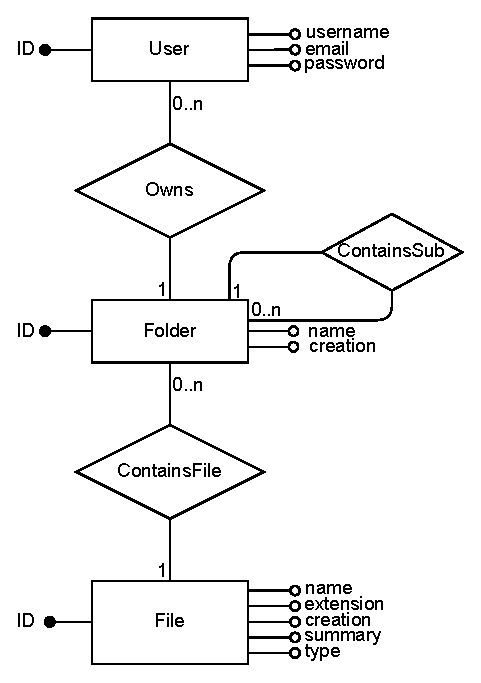
\includegraphics[width=0.7\columnwidth]{er}
		\end{center}
		
		\subsubsection{Logical schema}
		
		\verb|User (|\ulverb|id|\verb|,         | \grey{// [PK] User ID} \\
		\verb|      username,   | \grey{// Username} \\
		\verb|      email,      | \grey{// Email} \\
		\verb|      password)   | \grey{// Password} \\
		
		\verb|Folder (|\ulverb|id|\verb|,       | \grey{// [PK] Folder ID} \\
		\verb|        user,     | \grey{// [FK] Folder owner} \\
		\verb|        name,     | \grey{// Folder name} \\
		\verb|        creation, | \grey{// Folder creation date} \\
		\verb|        parent*)  | \grey{// Parent folder (if subfolder)} \\
		
		\verb|File (|\ulverb|id|\verb|,         | \grey{// [PK] File ID} \\
		\verb|      name,       | \grey{// File name} \\
		\verb|      extension,  | \grey{// File extension} \\
		\verb|      parent,     | \grey{// [FK] Parent folder ID} \\
		\verb|      creation,   | \grey{// Creation date} \\
		\verb|      summary,    | \grey{// File summary} \\
		\verb|      type)       | \grey{// File type}
		
	\end{multicols}
	
	\subsubsection{SQL}
	
	\begin{multicols}{2}
		\begin{minted}[samepage, tabsize=4]{SQL}
CREATE TABLE `User` (
	`id` int PRIMARY KEY,
	`username` varchar(45) NOT NULL,
	`email` varchar(45) NOT NULL,
	`password` varchar(45) NOT NULL
);
		\end{minted}
		\begin{minted}[samepage, tabsize=4]{SQL}
CREATE TABLE `Folder` (
	`id` int PRIMARY KEY,
	`user` int NOT NULL
		REFERENCES `User` (`id`)
		ON DELETE CASCADE
		ON UPDATE CASCADE,
	`name` varchar(45) NOT NULL,
	`creation` date NOT NULL,
	`parent` int DEFAULT NULL
		REFERENCES `Folder` (`id`)
		ON DELETE CASCADE
		ON UPDATE CASCADE
);
		\end{minted}
		\begin{minted}[samepage, tabsize=4]{SQL}
CREATE TABLE `File` (
	`id` int PRIMARY KEY,
	`name` varchar(45) NOT NULL,
	`extension` varchar(10) NOT NULL,
	`parent` int NOT NULL
		REFERENCES `Folder` (`id`)
		ON DELETE CASCADE
		ON UPDATE CASCADE,
	`creation` date NOT NULL,
	`summary` varchar(250) NOT NULL,
	`type` varchar(15) NOT NULL,
);
		\end{minted}
	\end{multicols}

	\pagebreak
	
	\subsection{Application design}
	
	\begin{center}
		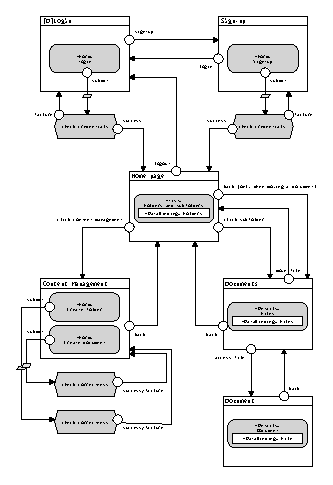
\includegraphics[width=0.95\columnwidth]{ifml}
	\end{center}
	
	\pagebreak
	
	\section{Components}
	
	\begin{multicols}{2}
		
		\subsection{Model objects (beans)}
		\begin{itemize}
			\item \verb|File|
			\item \verb|Folder|
			\item \verb|User|
		\end{itemize}
	
		\subsection{Data Access Objects (classes)}
		\begin{itemize}
			\item \verb|FileDAO|
			\begin{itemize}
				\item \verb|getFilesFromFolder|
				\item \verb|getFile|
				\item \verb|createFile|
				\item \verb|exists|
				\item \verb|moveFile|
			\end{itemize}
			\item \verb|FolderDAO|
			\begin{itemize}
				\item \verb|getFolder|
				\item \verb|getFoldersFromUser|
				\item \verb|exists|
				\item \verb|createFolder|
			\end{itemize}
			\item \verb|UserDAO|
			\begin{itemize}
				\item \verb|checkCredentials|
				\item \verb|exists|
				\item \verb|createUser|
			\end{itemize}
		\end{itemize}
		
		\subsection{Controllers (servlets)}
		
		\subsubsection{Frontend}
		\begin{itemize}
			\item \verb|File|
			\item \verb|Home|
			\item \verb|Login|
			\item \verb|MoveFile|
			\item \verb|NewItem|
			\item \verb|Signup|
			\item \verb|SubFolder|
		\end{itemize}
		
		\columnbreak
		
		\subsubsection{Backend}
		\begin{itemize}
			\item \verb|Controller|
			\item \verb|CreateFile|
			\item \verb|CreateFolder|
			\item \verb|Logout|
			\item \verb|MoveFile|
		\end{itemize}
	
		\subsection{Views (templates)}
		\begin{itemize}
			\item \verb|create.html|
			\item \verb|document.html|
			\item \verb|error.html|
			\item \verb|folder.html|
			\item \verb|home.html|
			\item \verb|login.html|
			\item \verb|moveFile.html|
			\item \verb|signup.html|
		\end{itemize}
		\vfill\null
	\end{multicols}
	
	\pagebreak
	
	\section{JavaScript}
	
	\begin{adjustwidth}{-30pt}{-30pt}
		\begin{center}
			\begin{tabular}{C|C|C|C|C|C}
				\multicolumn{3}{c|}{\textbf{Client side}} & \multicolumn{3}{c}{\textbf{Server side}} \\
				\centering \textbf{Event} & \centering \textbf{Action} & \centering \textbf{Controller} & \centering \textbf{Event} & \centering \textbf{Action} & \multicolumn{1}{c}{\textbf{Controller}} \\
				\hline
				login > form > submit & Data check & checkLogin() & POST username, password & Check validity & Login (servlet) \\
				\hline
				signup > form > submit & Data check & checkSignup() & POST username, mail, password, repeat password & Check validity & Signup (servlet) \\
				\hline
				home > load \#1 & View update with folders & home() & POST & Folders and subfolders search & Home (servlet) \\
				\hline
				home > load \#2 & View update with files & subfolder() & POST id & Check ownership and get files & SubFolder (servlet) \\
				\hline
				home > file > drop & Drop file into folder & dropFolder() & POST folderId, fileId & Check ownership and file movement & MoveFile (servlet) \\
				\hline
				home > file > drop & Drop file into recycle bin & dropBin() & $\times$ & $\times$ & $\times$ \\
				\hline
				home > file deletion modal > confirmation > click & File deletion modal confirmation & removeFile() & POST id & Check ownership and deletion & Deletion (servlet) \\
				\hline
				home > (sub)folder > drop & Drop folder into recycle bin & dropBin() & $\times$ & $\times$ & $\times$ \\
				\hline
				home > (sub)folder deletion modal > confirmation > click & Folder deletion modal confirmation & removeFolder() & POST id & Check ownership and deletion & Deletion (servlet) \\
				\hline
				home > file > click & Click on file & showFileDetails Modal() & POST id & Check ownership & File (servlet) \\
				\hline
				home > file add > click & Click on file creation & showFileModal() & $\times$ & $\times$ & $\times$ \\
				\hline
				home > file add modal > confirmation > click & Check data presence & createFile() & POST name, extension, parent, creation, summary, type & Check folder ownership, data validity and file creation & CreateFile (servlet) \\
				\hline
				home > subfolder add > click & Click on subfolder creation & showSubFolder Modal() & $\times$ & $\times$ & $\times$ \\
				\hline
				home > subfolder add modal > confirmation > click & Check data presence & createSubFolder() & POST name, parent, creation & Check data validity and file creation & CreateFolder (servlet) \\
				\hline
				home > folder add > click & Click on folder creation & showFolder Modal() & $\times$ & $\times$ & $\times$ \\
				\hline
				home > subfolder add modal > confirmation > click & Check data presence & createFolder() & POST name, parent, creation & Check folder ownership, data validity and file creation & CreateFolder (servlet) \\
				\hline
				home > logout > click & Logout & logout() & GET & User session deletion & Logout (servlet)
			\end{tabular}
		\end{center}
	\end{adjustwidth}
	
	\pagebreak
	
	\section{Events}
	
	\paragraph{Disclaimer} For simplicity, all the following diagrams represent only the case of well formatted requests and correct value, without errors. In reality, of course, everything is checked, at least server-side, and a proper error message is sent back to the client if anything goes wrong.
	
	\paragraph{Note} Items marked with \verb|[C]| are client-sided, while items marked with \verb|[S]| are server-sided.
	
	\subsection{Login}
	
	\paragraph{Pure HTML version}
	
	\begin{center}
		\begin{sequencediagram}
			\newthread{b}{[C] Browser}
			\newinst[0.8]{l}{[S] Login}
			\newinst[2.2]{u}{[S] UserDAO}
			\newinst{s}{[S] Session}
			
			\begin{call}{b}{POST}{l}{redirect(home)}
				\begin{call}{l}{checkCredentials(u, p)}{u}{User}
				\end{call}
				\begin{call}{l}{setAttribute(\doublequotes{user}, user)}{s}{}
				\end{call}
			\end{call}
		\end{sequencediagram}
	\end{center}
	
	\paragraph{RIA version}
	
	\begin{center}
		\begin{sequencediagram}
			\newthread{b}{[C] Browser}
			\newinst[1.2]{w}{[C] window}
			\newinst{ss}{[C] sessionStorage}
			\newinst{l}{[S] Login}
			\newinst[1.9]{u}{[S] UserDAO}
			\newinst{s}{[S] Session}
			
			\begin{call}{b}{POST}{l}{200}
				\begin{call}{l}{checkCredentials(u, p)}{u}{User}
				\end{call}
				\begin{call}{l}{setAttribute(\doublequotes{user}, user)}{s}{}
				\end{call}
			\end{call}
			\begin{call}{b}{setItem(\doublequotes{username}, username)}{ss}{}
			\end{call}
			\begin{call}{b}{location = /home/}{w}{}
			\end{call}
		\end{sequencediagram}
	\end{center}
	
	\pagebreak
	
	\subsection{Sign-up}
	
	\paragraph{Pure HTML version}
	
	\begin{center}
		\begin{sequencediagram}
			\newthread{b}{[C] Browser}
			\newinst[0.7]{s}{[S] Signup}
			\newinst[1.2]{u}{[S] UserDAO}
			\newinst{se}{[S] Session}
			
			\begin{call}{b}{POST}{s}{redirect(home)}
				\begin{call}{s}{exists(username)}{u}{false}
				\end{call}
				\begin{call}{s}{createUser(u, e, p)}{u}{User}
				\end{call}
				\begin{call}{s}{setAttribute(\doublequotes{user}, user)}{se}{}
				\end{call}
			\end{call}
		\end{sequencediagram}
	\end{center}
	
	\paragraph{RIA version}
	
	\begin{center}
		\begin{sequencediagram}
			\newthread{b}{[C] Browser}
			\newinst[1.2]{w}{[C] window}
			\newinst{ss}{[C] sessionStorage}
			\newinst{s}{[S] Signup}
			\newinst[1.2]{u}{[S] UserDAO}
			\newinst{se}{[S] Session}
			
			\begin{call}{b}{POST}{s}{200}
				\begin{call}{s}{exists(username)}{u}{false}
				\end{call}
				\begin{call}{s}{createUser(u, e, p)}{u}{User}
				\end{call}
				\begin{call}{s}{setAttribute(\doublequotes{user}, user)}{se}{}
				\end{call}
			\end{call}
			\begin{call}{b}{setItem(\doublequotes{username}, username)}{ss}{}
			\end{call}
			\begin{call}{b}{location = /home/}{w}{}
			\end{call}
		\end{sequencediagram}
	\end{center}
	
	\pagebreak
	
	\subsection{Home page access}
	
	\paragraph{Pure HTML version}
	
	\begin{center}
		\begin{sequencediagram}
			\newthread{u}{[C] Browser}
			\newinst{h}{[S] HomePage}
			\newinst[2.2]{f}{[S] FolderDAO}
			\newinst{c}{[S] WebContext}
			\newinst{e}{[S] TemplateEngine}
			
			\begin{call}{u}{GET}{h}{home.html}
				\begin{call}{h}{getFoldersFromUser(user)}{f}{folders}
				\end{call}
				\begin{call}{h}{setVariable(\doublequotes{folders}, subFolders)}{c}{}
				\end{call}
				\begin{call}{h}{process(html)}{e}{}
				\end{call}
			\end{call}
		\end{sequencediagram}
	\end{center}
	
	\paragraph{RIA version}
	
	\begin{center}
		\begin{sequencediagram}
			\newthread{u}{[C] Browser}
			\newinst{d}{[C] document}
			\newinst{h}{[S] HomePage}
			\newinst{fc}{[S] Subfolder}
			\newinst{f}{[S] FolderDAO}
			\newinst{fi}{[S] FileDAO}
			
			\begin{call}{u}{GET}{h}{home.html}
			\end{call}
			
			\begin{call}{u}{POST}{h}{json}
				\begin{call}{h}{getFoldersFromUser(user)}{f}{folders}
				\end{call}
				\begin{call}{h}{prepareJson()}{h}{json}
				\end{call}
			\end{call}
			
			\begin{sdblock}{loop}{for each subfolder sf}
				\begin{call}{u}{POST}{fc}{json}
					\begin{call}{fc}{getFilesFromFolder(sf)}{fi}{files}
					\end{call}
					\begin{call}{fc}{prepareJson()}{fc}{json}
					\end{call}
				\end{call}
			\end{sdblock}
			
			\begin{call}{u}{resetFields()}{d}{}
			\end{call}
			\begin{call}{u}{show(json)}{d}{}
			\end{call}
		\end{sequencediagram}
	\end{center}
	
	\pagebreak
	
	\subsection{Subfolder access}
	
	\paragraph{Pure HTML version}
	
	\begin{center}
		\begin{sequencediagram}
			\newthread{u}{[C] Browser}
			\newinst{h}{[S] SubFolder}
			\newinst{f}{[S] FolderDAO}
			\newinst{fi}{[S] FileDAO}
			\newinst{c}{[S] WebContext}
			\newinst{e}{[S] TemplateEngine}
			
			\begin{call}{u}{GET}{h}{folder.html}
				\begin{call}{h}{getFolder(id)}{f}{folder}
				\end{call}
				\begin{call}{h}{getFilesFromFolder(id)}{fi}{files}
				\end{call}
				\begin{call}{h}{setVariable(\doublequotes{files}, files)}{c}{}
				\end{call}
				\begin{call}{h}{setVariable(\doublequotes{folderName}, folder.getName())}{c}{}
				\end{call}
				\begin{call}{h}{process(html)}{e}{}
				\end{call}
			\end{call}
		\end{sequencediagram}
	\end{center}
	
	\paragraph{RIA version} There is no correspondence between the pure HTML version and the RIA version, because in this case it's merged into the home page displaying process.
	
	\pagebreak
	
	\subsection{Document access}
	
	\paragraph{Pure HTML version}
	
	\begin{center}
		\begin{sequencediagram}
			\newthread{u}{[C] Browser}
			\newinst[0.8]{h}{[S] File}
			\newinst{fi}{[S] FileDAO}
			\newinst{f}{[S] FolderDAO}
			\newinst[0.7]{c}{[S] WebContext}
			\newinst{e}{[S] TemplateEngine}
			
			\begin{call}{u}{GET}{h}{document.html}
				\begin{call}{h}{getFile(id)}{fi}{file}
				\end{call}
				\begin{call}{h}{getFolder(file.getParent())}{f}{sf}
				\end{call}
				\begin{call}{h}{getFolder(sf.getParent())}{f}{f}
				\end{call}
				\begin{call}{h}{setVariable(\doublequotes{folder}, /f.getName()/sf.getName())}{c}{}
				\end{call}
				\begin{call}{h}{setVariable(\doublequotes{document}, file)}{c}{}
				\end{call}
				\begin{call}{h}{process(html)}{e}{}
				\end{call}
			\end{call}
		\end{sequencediagram}
	\end{center}
	
	\paragraph{RIA version}
	
	\begin{center}
		\begin{sequencediagram}
			\newthread{u}{[C] Browser}
			\newinst{d}{[C] document}
			\newinst{h}{[S] File}
			\newinst{fi}{[S] FileDAO}
			\newinst{f}{[S] FolderDAO}
			
			\begin{call}{u}{POST}{h}{json}
				\begin{call}{h}{getFile(id)}{fi}{file}
				\end{call}
				\begin{call}{h}{getFolder(file.getParent())}{f}{sf}
				\end{call}
				\begin{call}{h}{getFolder(sf.getParent())}{f}{f}
				\end{call}
				\begin{call}{h}{prepareJson()}{h}{json}
				\end{call}
			\end{call}
			
			\begin{call}{u}{resetFields()}{d}{}
			\end{call}
			\begin{call}{u}{show(json)}{d}{}
			\end{call}
		\end{sequencediagram}
	\end{center}
	
	\pagebreak
	
	\subsection{File creation}
	
	\paragraph{Pure HTML version}
	
	\begin{center}
		\begin{sequencediagram}
			\newthread{u}{[C] Browser}
			\newinst[0.4]{h}{[S] CreateFile}
			\newinst[0.4]{fi}{[S] FileDAO}
			\newinst[0.4]{f}{[S] FolderDAO}
			\newinst{c}{[S] WebContext}
			\newinst{e}{[S] TemplateEngine}
			
			\begin{sdblock}{conditional}{file doesn't already exists}
				\begin{call}{u}{POST}{h}{redirect(home)}
					\begin{call}{h}{exists(file)}{fi}{false}
					\end{call}
					\begin{call}{h}{getFolder(parent)}{f}{parent}
					\end{call}
					\begin{call}{h}{createFile(file)}{fi}{}
					\end{call}
				\end{call}
			\end{sdblock}
			\begin{sdblock}{conditional}{file already exists}
				\begin{call}{u}{POST}{h}{create.html}
					\begin{call}{h}{exists(file)}{fi}{true}
					\end{call}
					\begin{call}{h}{getFoldersFromUser(user)}{f}{folders}
					\end{call}
					\begin{call}{h}{setVariable(\doublequotes{errorMessageFile}, \doublequotes{error})}{c}{}
					\end{call}
					\begin{call}{h}{setVariable(\doublequotes{folders}, folders)}{c}{}
					\end{call}
					\begin{call}{h}{setVariable(\doublequotes{subfolders}, subfolders)}{c}{}
					\end{call}
					\begin{call}{h}{process(html)}{e}{}
					\end{call}
				\end{call}
			\end{sdblock}
		\end{sequencediagram}
	\end{center}
	
	\pagebreak
	
	\paragraph{RIA version}
	
	\begin{center}
		\begin{sequencediagram}
			\newthread{u}{[C] Browser}
			\newinst{d}{[C] document}
			\newinst{w}{[C] window}
			\newinst{h}{[S] CreateFile}
			\newinst[0.4]{fi}{[S] FileDAO}
			\newinst[0.4]{f}{[S] FolderDAO}
			
			\begin{sdblock}{conditional}{file doesn't already exists}
				\begin{call}{u}{POST}{h}{200}
					\begin{call}{h}{exists(file)}{fi}{false}
					\end{call}
					\begin{call}{h}{getFolder(parent)}{f}{parent}
					\end{call}
					\begin{call}{h}{createFile(file)}{fi}{}
					\end{call}
				\end{call}
			\end{sdblock}
			\begin{sdblock}{conditional}{file already exists}
				\begin{call}{u}{POST}{h}{error}
					\begin{call}{h}{exists(file)}{fi}{true}
					\end{call}
				\end{call}
				\begin{call}{u}{show(error)}{d}{}
				\end{call}
			\end{sdblock}
		\end{sequencediagram}
	\end{center}
	
	\pagebreak
	
	\subsection{Folder creation}
	
	\paragraph{Pure HTML version}
	
	\begin{center}
		\begin{sequencediagram}
			\newthread{u}{[C] Browser}
			\newinst[0.4]{h}{[S] CreateFolder}
			\newinst[1.8]{f}{[S] FolderDAO}
			\newinst{c}{[S] WebContext}
			\newinst{e}{[S] TemplateEngine}
			
			\begin{sdblock}{conditional}{folder doesn't already exists}
				\begin{call}{u}{POST}{h}{redirect(home)}
					\begin{call}{h}{exists(folder)}{f}{false}
					\end{call}
					\begin{call}{h}{createFolder(folder)}{f}{}
					\end{call}
				\end{call}
			\end{sdblock}
			\begin{sdblock}{conditional}{folder already exists}
				\begin{call}{u}{POST}{h}{create.html}
					\begin{call}{h}{exists(folder)}{f}{true}
					\end{call}
					\begin{call}{h}{getFoldersFromUser(user)}{f}{folders}
					\end{call}
					\begin{call}{h}{setVariable(\doublequotes{errorMessageFolder}, \doublequotes{error})}{c}{}
					\end{call}
					\begin{call}{h}{setVariable(\doublequotes{folders}, folders)}{c}{}
					\end{call}
					\begin{call}{h}{setVariable(\doublequotes{subfolders}, subfolders)}{c}{}
					\end{call}
					\begin{call}{h}{process(html)}{e}{}
					\end{call}
				\end{call}
			\end{sdblock}
		\end{sequencediagram}
	\end{center}
	
	\pagebreak
	
	\paragraph{RIA version}
	
	\begin{center}
		\begin{sequencediagram}
			\newthread{u}{[C] Browser}
			\newinst{d}{[C] document}
			\newinst{w}{[C] window}
			\newinst{h}{[S] CreateFolder}
			\newinst[0.8]{f}{[S] FolderDAO}
			
			\begin{sdblock}{conditional}{folder doesn't already exists}
				\begin{call}{u}{POST}{h}{200}
					\begin{call}{h}{exists(folder)}{f}{false}
					\end{call}
					\begin{call}{h}{createFolder(folder)}{f}{}
					\end{call}
				\end{call}
			\end{sdblock}
			\begin{sdblock}{conditional}{folder already exists}
				\begin{call}{u}{POST}{h}{error}
					\begin{call}{h}{exists(folder)}{f}{true}
					\end{call}
				\end{call}
				\begin{call}{u}{show(error)}{d}{}
				\end{call}
			\end{sdblock}
		\end{sequencediagram}
	\end{center}
	
	\pagebreak
	
	\subsection{File movement}
	
	\paragraph{Pure HTML version}
	
	\begin{center}
		\begin{sequencediagram}
			\newthread{u}{[C] Browser}
			\newinst{h}{[S] f/MoveFile}
			\newinst{h1}{[S] b/MoveFile}
			\newinst{f}{[S] FolderDAO}
			\newinst{fi}{[S] FileDAO}
			\newinst{c}{[S] W.C.}
			\newinst{e}{[S] T.E.}
			
			\begin{call}{u}{GET}{h}{moveFile.html}
				\begin{call}{h}{getFile(id)}{fi}{file}
				\end{call}
				\begin{call}{h}{getFoldersFromUser(user)}{f}{folders}
				\end{call}
				\begin{call}{h}{getFolder(file.parent())}{f}{source}
				\end{call}
				\begin{call}{h}{setVariable(\doublequotes{folders}, folders)}{c}{}
				\end{call}
				\begin{call}{h}{setVariable(\doublequotes{source}, source)}{c}{}
				\end{call}
				\begin{call}{h}{setVariable(\doublequotes{moving\_file}, file)}{c}{}
				\end{call}
				\begin{call}{h}{process(html)}{e}{}
				\end{call}
			\end{call}
			
			\begin{call}{u}{GET}{h1}{redirect(destination)}
				\begin{call}{h1}{getFile(fiID)}{fi}{file}
				\end{call}
				\begin{call}{h1}{getFolder(foID)}{f}{destination}
				\end{call}
				\begin{call}{h1}{moveFile(file, destination)}{fi}{}
				\end{call}
			\end{call}
		\end{sequencediagram}
	\end{center}
	
	\paragraph{RIA version}
	
	\begin{center}
		\begin{sequencediagram}
			\newthread{u}{[C] Browser}
			\newinst{h}{[S] MoveFile}
			\newinst[0.5]{f}{[S] FolderDAO}
			\newinst{fi}{[S] FileDAO}
			
			\begin{call}{u}{POST}{h}{200}
				\begin{call}{h}{getFile(fiID)}{fi}{file}
				\end{call}
				\begin{call}{h}{getFolder(foID)}{f}{destination}
				\end{call}
				\begin{call}{h}{moveFile(file, destination)}{fi}{}
				\end{call}
			\end{call}
		\end{sequencediagram}
	\end{center}
	
	\pagebreak
	
	\subsection{Deletion}
	
	\paragraph{Pure HTML version} In this version there is no file or folder deletion.
	
	\paragraph{RIA version}
	
	\begin{center}
		\begin{sequencediagram}
			\newthread{u}{[C] Browser}
			\newinst{h}{[S] Deletion}
			\newinst{f}{[S] FolderDAO}
			\newinst{fi}{[S] FileDAO}
			
			\begin{call}{u}{POST}{h}{200}
				\begin{sdblock}{conditional}{folder deletion}
					\begin{call}{h}{getFolder(id)}{f}{folder}
					\end{call}
					\begin{call}{h}{delete(id)}{f}{}
					\end{call}
				\end{sdblock}
				\begin{sdblock}{conditional}{file deletion}
					\begin{call}{h}{getFile(id)}{fi}{file}
					\end{call}
					\begin{call}{h}{delete(id)}{fi}{}
					\end{call}
				\end{sdblock}
			\end{call}
		\end{sequencediagram}
	\end{center}

\end{document}
